% THIS IS SIGPROC-SP.TEX - VERSION 3.1
% WORKS WITH V3.2SP OF ACM_PROC_ARTICLE-SP.CLS
% APRIL 2009
%
% It is an example file showing how to use the 'acm_proc_article-sp.cls' V3.2SP
% LaTeX2e document class file for Conference Proceedings submissions.
% ----------------------------------------------------------------------------------------------------------------
% This .tex file (and associated .cls V3.2SP) *DOES NOT* produce:
%       1) The Permission Statement
%       2) The Conference (location) Info information
%       3) The Copyright Line with ACM data
%       4) Page numbering
% ---------------------------------------------------------------------------------------------------------------
% It is an example which *does* use the .bib file (from which the .bbl file
% is produced).
% REMEMBER HOWEVER: After having produced the .bbl file,
% and prior to final submission,
% you need to 'insert'  your .bbl file into your source .tex file so as to provide
% ONE 'self-contained' source file.
%
% Questions regarding SIGS should be sent to
% Adrienne Griscti ---> griscti@acm.org
%
% Questions/suggestions regarding the guidelines, .tex and .cls files, etc. to
% Gerald Murray ---> murray@hq.acm.org
%
% For tracking purposes - this is V3.1SP - APRIL 2009

\documentclass{acm_proc_article-sp}

\begin{document}

\title{Title!!!!!!!!!}
%
% You need the command \numberofauthors to handle the 'placement
% and alignment' of the authors beneath the title.
%
% For aesthetic reasons, we recommend 'three authors at a time'
% i.e. three 'name/affiliation blocks' be placed beneath the title.
%
% NOTE: You are NOT restricted in how many 'rows' of
% "name/affiliations" may appear. We just ask that you restrict
% the number of 'columns' to three.
%
% Because of the available 'opening page real-estate'
% we ask you to refrain from putting more than six authors
% (two rows with three columns) beneath the article title.
% More than six makes the first-page appear very cluttered indeed.
%
% Use the \alignauthor commands to handle the names
% and affiliations for an 'aesthetic maximum' of six authors.
% Add names, affiliations, addresses for
% the seventh etc. author(s) as the argument for the
% \additionalauthors command.
% These 'additional authors' will be output/set for you
% without further effort on your part as the last section in
% the body of your article BEFORE References or any Appendices.

\numberofauthors{5} %  in this sample file, there are a *total*
% of EIGHT authors. SIX appear on the 'first-page' (for formatting
% reasons) and the remaining two appear in the \additionalauthors section.
%
\author{
% You can go ahead and credit any number of authors here,
% e.g. one 'row of three' or two rows (consisting of one row of three
% and a second row of one, two or three).
%
% The command \alignauthor (no curly braces needed) should
% precede each author name, affiliation/snail-mail address and
% e-mail address. Additionally, tag each line of
% affiliation/address with \affaddr, and tag the
% e-mail address with \email.
%
% 1st. author
\alignauthor
Yan Songyang\\
       \affaddr{School of Software Engneering}\\
       \affaddr{Xi'an Jiaotong University}\\
       \email{lapalacayim@gmail.com}
% 2nd. author
\alignauthor
Li Siyu\\
       \affaddr{College of Cybersecurity}\\
       \affaddr{Sichuan University}\\
       \email{sy\_lee\_real@icloud.com}
% 3rd. author
\alignauthor Wan Ziyi\\
       \affaddr{College of Cybersecurity}\\
       \affaddr{Sichuan University}\\
       \email{scuderrickwan@gmail.com}
\and  % use '\and' if you need 'another row' of author names
% 4th. author
\alignauthor Ye Junyan\\
       \affaddr{School of Information and Software Engineering}\\
       \affaddr{University of Electronic Science and Technology}\\
       \email{2239308357@qq.com}
% 5th. author
\alignauthor Li Hanxing\\
       \affaddr{School of Cyber Science and Engineering}\\
       \affaddr{Wuhan University}\\
       \email{t0918555@u.nus.edu}
}
% There's nothing stopping you putting the seventh, eighth, etc.
% author on the opening page (as the 'third row') but we ask,
% for aesthetic reasons that you place these 'additional authors'
% in the \additional authors block, viz.
% Just remember to make sure that the TOTAL number of authors
% is the number that will appear on the first page PLUS the
% number that will appear in the \additionalauthors section.

\maketitle
\begin{abstract}
Abstract here
\end{abstract}

% A category with the (minimum) three required fields
\category{H.4}{Input/Output and Data Communications}{Data Communication Devices}


\terms{Theory}

\keywords{Drone, Remote Control} % NOT required for Proceedings

\section{Introduction}

 The drone, also known as the unmanned aerial vehicle(UAV), is the Aircraft without  any human pilot controlling inside. Drones are widely used in many fields, including military, industry, agriculture, photography and so on. We can simply divide them into civilian and military. 
 
 The civilian drones, which we are focusing on, are applied to countless aspects of our lives.  Farmers use drones to spray pesticides and monitor crop's growth. E-commerce companies such as Amazon use drones to deliver express. Photographers use drones to create from a special perspective. And also people, just like us, using drones just for fun. All in all, the use of drones has penetrated into many aspect of our lives.
 
  Quadcopter, one of the most common types of civilian drones, using Wi-Fi connection or 2.4GHz radio as its way of communication, generally. Some professional drone companies such as DJI may have their own private communication protocols and they are beyond our research.
  
 Within Wi-Fi connection, a drone is WLAN AP(Access Point) itself. If the user wants to control the drone, he needs to connect his smartphone(or other smart devices) with control application to the WLAN created by the drone. And there may be steps to authenticate during the connection establishment process. Then user’s smartphone could issue instructions to the drone and receive real-time image transmission from drone, after getting the Wi-Fi connection to the drone.
 
 And the other way of communication is using 2.4GHz radio. This is a much simpler communication mechanism, which means it has a lower cost and usually used on low-end drones. 2.4GHz radio technique is widely used in lots of remote controls, and remote control used in toys including drones is the one of the application scenarios. The remote control sending instructions via an agreed frequency in 2.4GHz ISM, and the drone receive these instructions. The massage transmit via 2.4GHz radio broadcasts to anyone that can receive it, which means there isn’t any connection between remote control and the drone. Not to mention identity verification. So this is a primitive way of control, which is easy to attack.

\section{Attack on the AR.Drone 2.0}

\subsection{Technical Specification}
The AR.Drone 2.0, equipped with various sensors, uses a Linux operating system based on the kernel version 2.6.27.44. All control commands, telemetry data and the video streams are handled via (unencrypted) 2.4GHz WLAN communication with the controlling device. Users can use iOS and Android devices to control the drone via the official application AR.FreeFlight. Figure ~\ref{iPad} shows the controller interface running on iPad.

\begin{figure}
\centering
\label{iPad}
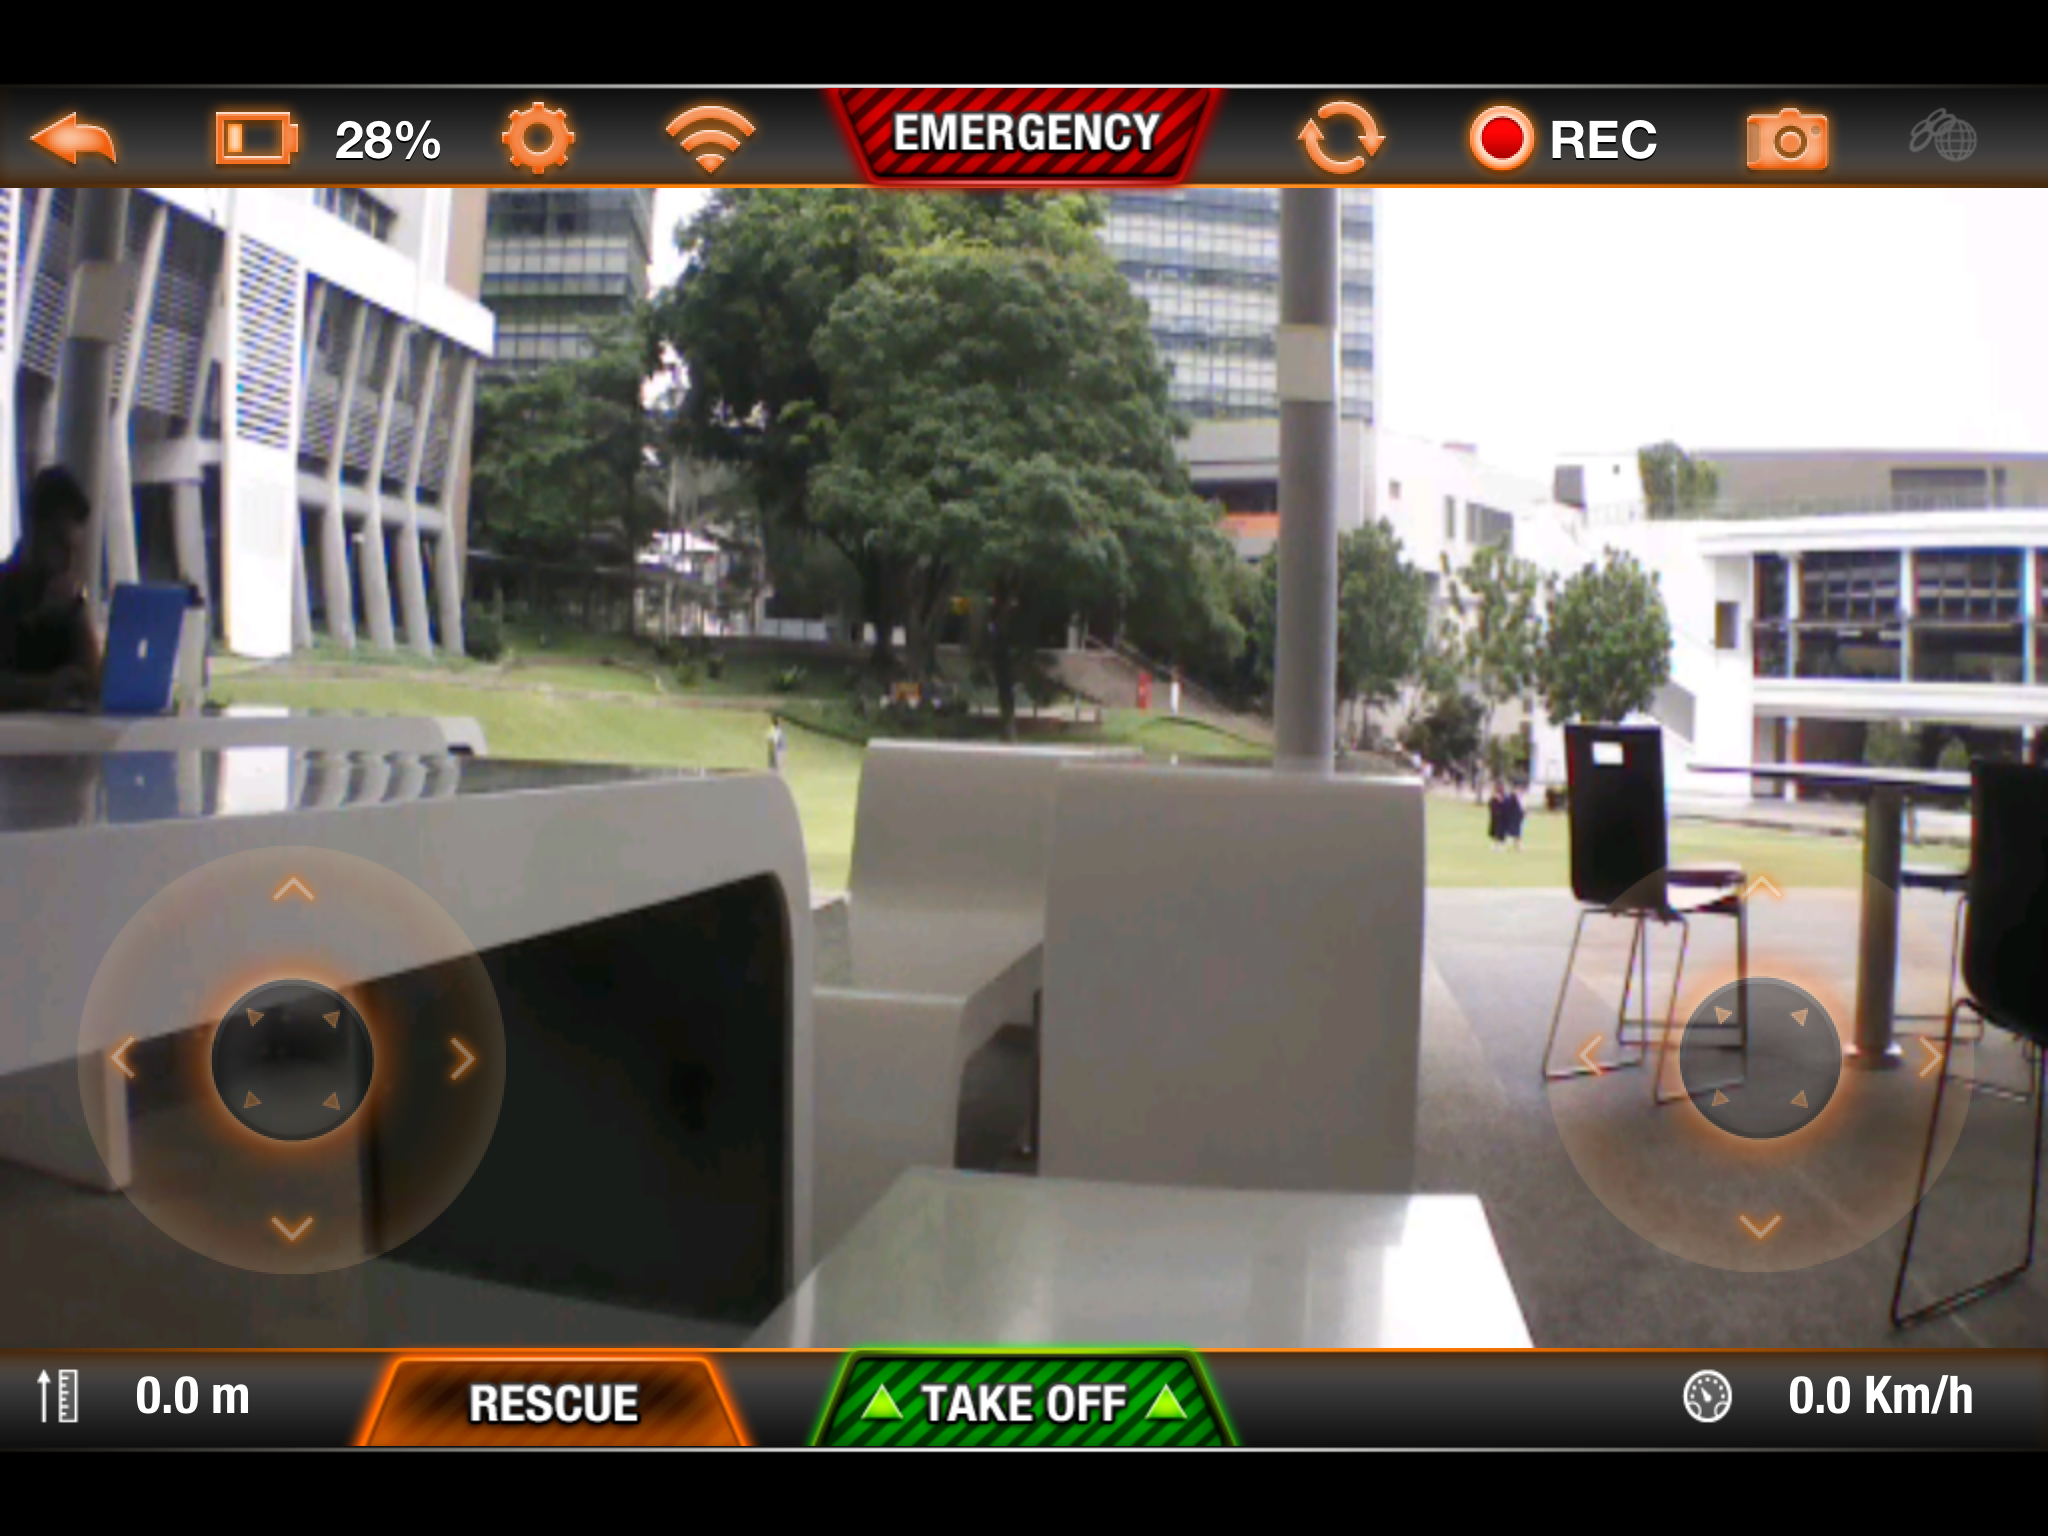
\epsfig{file=figures/iPad.PNG, height=1.2in, width=1.8in}
\caption{Parrot AR.FreeFlight control interface}
\end{figure}


\subsection{Highjack Attack}

\subsubsection{AT Commands}
According to AR.Drone Developer Guide\cite{dev:guide}, the controller uses port 5556 to send commands in a UDP packet to port 5556 of the drone. These commands are called AT commands. Because of the instability of UDP connection, the communication protocol allocates ascending sequence number to different commands. This prevents older commands with lower sequence numbers incoming later (due to transmission errors) from executing\cite{hack:secure}. This protocol provides an attack method. Attacker can conduct a man-in-the-middle attack with a sequence number which is always higher than the one being sent from the legitimate user.

An AT command begins with the fixed string "AT*", followed by either REF, PCMD or CONFIG. REF commands are single commands such as land or takeoff. PCMD commands are used for flight control. CONFIG commands are used for sending new configuration. To take over a drone, using REF commands is enough. As described in\cite{dev:guide}, the format command of REF command is 

\begin{equation}
  AT*REF=<sequence>,<UI>
\end{equation}


Different REF commands are listed in table ~\ref{refcom}.

\begin{table}
\centering
\caption{REF commands}
\label{refcom}
\begin{tabular}{@{}ll@{}} \hline
Command                                            & Function       \\ \hline
AT\*REF=\textless{}sequence\textgreater{},290718208 & Take off       \\ \hline
AT\*REF=\textless{}sequence\textgreater{},290717696 & Land           \\ \hline
AT\*REF=\textless{}sequence\textgreater{},290717952 & Emergency Stop \\ \hline
\end{tabular}
\end{table}


\subsubsection{Attack Process}

The attack consists of the following phases:

\begin{enumerate}
  \item Connection to the drone,
  \item Determination of the IP address of the control device,
  \item Sending fake land packets with high sequence number.
\end{enumerate}

After booting up, the drone will set up a Wi-Fi hotspot named "ardrone2\_" followed by a random number with 6 digits. The connection to the drone is possible because the network is not protected by any encryption or other access restriction techniques. The ip address of the drone itself is always 192.168.1.1/24.

Once the connection has been built, attacker can scan the subnetwork to determine the IP address of the control device.

To prevent multiple phones trying to control the drone, the drone only accepts packets from the source IP of the controller. But since it's UDP, it's simple to spoof the IP address of the controller. Attacker can send a land command to force the drone to come to the ground.\cite{drone:python}

\subsubsection{Using Android Device to Conduct Attack}

After the previous analysis, we have mastered the WIFI-controlled drone attack method and the whole process. The drone uses the application(FreeFlight 2.0) to control takeoff, landing, flight direction and capture image acquisition. We decided to create another Android application to attack this drone. Then this application can be controlled by a third party and take control of the drone, force the drone to land, and modify the flight direction.

The attack consists of the following phases:

\begin{enumerate}
  \item The third-party user uses the Android packet capture application to obtain the target drone IP address,
  \item After the third-party user enters the obtained IP address in this application, he can click the button to send a command to control the drone.
\end{enumerate}


Jpcap provides a class JpcapSender for sending packets, which can be used to send IPPackets and its subclasses, including IPPacket, ICMPPacket, TCPPacket, UDPPacket\cite{jpcap}. After defining a corresponding package, we can use the SendPacket function to send packets. Meanwhile, Jpcap can be used to construct IP data packets to implement sending fake IP.

The creation of this new Android app is primarily convenient for any third-party user who can hijack drones directly at the application layer.



\section{Attack on hubsan blablabla}

//TODO

\section{Discussions}

gugugu


\section{Conclusions}

We..... and....., however... it's..... great!

%\end{document}  % This is where a 'short' article might terminate

%ACKNOWLEDGMENTS are optional
\section{Acknowledgments}

We would like to offer our sincere appreciation and thanks to Professor Hugh Anderson for his guidance, enthusiasm and encouragement during the project. He is always generous in providing all kinds of equipment we might need and we are equally grateful to the School of Computing for this. And we also thank our teaching assistant Tan Wang Leng for his insight and expertise. Without them, we wouldn't have gone thus far.

%
% The following two commands are all you need in the
% initial runs of your .tex file to
% produce the bibliography for the citations in your paper.
\bibliographystyle{abbrv}
\bibliography{sigproc}  % sigproc.bib is the name of the Bibliography in this case
% You must have a proper ".bib" file
%  and remember to run:
% latex bibtex latex latex
% to resolve all references
%
% ACM needs 'a single self-contained file'!
%
%APPENDICES are optional
%\balancecolumns

\balancecolumns
% That's all folks!
\end{document}
